% Options for packages loaded elsewhere
\PassOptionsToPackage{unicode}{hyperref}
\PassOptionsToPackage{hyphens}{url}
%
\documentclass[
]{article}
\usepackage{lmodern}
\usepackage{amssymb,amsmath}
\usepackage{ifxetex,ifluatex}
\ifnum 0\ifxetex 1\fi\ifluatex 1\fi=0 % if pdftex
  \usepackage[T1]{fontenc}
  \usepackage[utf8]{inputenc}
  \usepackage{textcomp} % provide euro and other symbols
\else % if luatex or xetex
  \usepackage{unicode-math}
  \defaultfontfeatures{Scale=MatchLowercase}
  \defaultfontfeatures[\rmfamily]{Ligatures=TeX,Scale=1}
\fi
% Use upquote if available, for straight quotes in verbatim environments
\IfFileExists{upquote.sty}{\usepackage{upquote}}{}
\IfFileExists{microtype.sty}{% use microtype if available
  \usepackage[]{microtype}
  \UseMicrotypeSet[protrusion]{basicmath} % disable protrusion for tt fonts
}{}
\makeatletter
\@ifundefined{KOMAClassName}{% if non-KOMA class
  \IfFileExists{parskip.sty}{%
    \usepackage{parskip}
  }{% else
    \setlength{\parindent}{0pt}
    \setlength{\parskip}{6pt plus 2pt minus 1pt}}
}{% if KOMA class
  \KOMAoptions{parskip=half}}
\makeatother
\usepackage{xcolor}
\IfFileExists{xurl.sty}{\usepackage{xurl}}{} % add URL line breaks if available
\IfFileExists{bookmark.sty}{\usepackage{bookmark}}{\usepackage{hyperref}}
\hypersetup{
  pdftitle={Donald Trump May Win His Re-election Campaign?},
  pdfauthor={Yijie Zhao, Yifan Xu, Yuyan Xu \& Yuze Kang},
  hidelinks,
  pdfcreator={LaTeX via pandoc}}
\urlstyle{same} % disable monospaced font for URLs
\usepackage[margin=1in]{geometry}
\usepackage{graphicx,grffile}
\makeatletter
\def\maxwidth{\ifdim\Gin@nat@width>\linewidth\linewidth\else\Gin@nat@width\fi}
\def\maxheight{\ifdim\Gin@nat@height>\textheight\textheight\else\Gin@nat@height\fi}
\makeatother
% Scale images if necessary, so that they will not overflow the page
% margins by default, and it is still possible to overwrite the defaults
% using explicit options in \includegraphics[width, height, ...]{}
\setkeys{Gin}{width=\maxwidth,height=\maxheight,keepaspectratio}
% Set default figure placement to htbp
\makeatletter
\def\fps@figure{htbp}
\makeatother
\setlength{\emergencystretch}{3em} % prevent overfull lines
\providecommand{\tightlist}{%
  \setlength{\itemsep}{0pt}\setlength{\parskip}{0pt}}
\setcounter{secnumdepth}{-\maxdimen} % remove section numbering

\title{Donald Trump May Win His Re-election Campaign?}
\usepackage{etoolbox}
\makeatletter
\providecommand{\subtitle}[1]{% add subtitle to \maketitle
  \apptocmd{\@title}{\par {\large #1 \par}}{}{}
}
\makeatother
\subtitle{Prediction on 2020 US Presidential Election}
\author{Yijie Zhao, Yifan Xu, Yuyan Xu \& Yuze Kang}
\date{1 November 2020}

\begin{document}
\maketitle
\begin{abstract}
In this paper, we use survey data from Democracy Fund + UCLA Nationscape
to build regression model. We apply this model to census sample data
from IPUMS USA by using multilevel regression with post-stratification.
We predict that Donald Trump wins 45.4\% of the national popular vote
and lose his re-election campaign..\\
~\\
\textbf{Keywords:} Forecasting; US 2020 Election; Trump; Biden;
Multilevel Regression with Post-stratification.
\end{abstract}

\hypertarget{introduction}{%
\section{Introduction}\label{introduction}}

The presidential election campaign is held every four years. Before the
official campaign day, American political analysts and scholars
typically spent hours dedicating in forecasting the winner of election.
This is a national matter such that every U.S. citizen deeply cares
about. The last election in 2016, Donald Trump lost the popular vote
against Hillary Clinton but still won the election and became the new
U.S. president. His vote share was mostly located in the rural and
suburban areas, where he won 70\% of the popular vote; Clinton on the
other hand, had a vote share located in densely populated areas (Hennig,
2017). Although Clinton won the popular vote, the winning majority in
the Electoral College leaned towards the republican candidate, as a
result, Trump won by securing the votes in some of the important swing
states (Hennig, 2017). This year, the U.S. election seems more
intriguing and uncertain under the shadows of COVID-19. The two
candidates that have dominant polling are Donald Trump and the
Democratic presidential nominee Joe Biden. Polling research have
observed that the American voters changed their concerns and behaviour
due to the effects of COVID-19, their major concern were the economy
(Zhang \& Fedor, 2020). The October polling showed that about 53 percent
of Democrats believed they were worse off financially since Trump became
president and 9 percent of Republicans do (Zhang \& Fedor, 2020). This
shows that voters are starting to reconsider their choices of candidate
because the pandemic has brought doubts and criticisms on Trump's policy
on dealing with the spreading of the disease. However, the lap in
national polls does not mean that Trump will lose the election on
November 3. This report is in an effort to predict the outcome of
election by constructing statistical models to analyze the current
voting trend. We eliminated the other candidates and only consider the
two candidates with dominant polling, Donald Trump and Joe Biden. Our
objective is to discover the voter's behaviour and how they think of
Donald Trump, and then predict the chance of Donald Trump win the 2020
election by using these analytic findings.

In this report, we used the first release of the Phase 2 data in August
2020 from UCLA Nationalscape as our survey data. The dataset we chose
was the wave 50 of the Nationalscape data (20200625). In addition to
this, we also used the 2018 census data from American Community Surveys
(ACS) as our post-stratification data. Post-stratification is an
statistical method that allows adjusting the samples in order to match
the general population. When conducting the survey, pollsters often need
to deal with nonresponse from the potential respondents. These
nonresponses could contribute to a bias on the research findings such
that they cannot reflect on the real large population.
Post-stratification is a way to deal with the nonresponse situation. In
this survey, we first cleaned the data by identifying any errors in the
data and removed them. In the data section, we used bar plots and
histograms to analyze the demographic information about the voters who
voted Donald Trump in each dataset.

We then construct a linear regression model on the survey data to
observe the response (people voting Trump) and predictor variables
(voter's age, sex, and race), then apply the predictive model on the
census data to make prediction on the probability of each state voting
Trump. The reason we focused on the polling probability in states is, a
candidate must win at least 270 votes in electoral college in order to
be elected as the U.S. president. Each U.S. state gets a certain number
of votes in electoral college based on its population. By looking up on
these statistics allow us to make better predictions on the chances that
Trump wins this election. During this process, we found that Maine
(51.8\%), Montana (52.5\%), New Mexico (51.5\%) and Vermont (52.9\%)
have the highest probability of voting Trump in electoral college. It is
worth mentioning that the swing states such as Arizona has a 47.9\%,
Minnesota has a 41\%, Florida has a 46.7\%. In addition, the prediction
on overall national polls is that about 49\% of the voters would vote
for Trump, 51\% of the voters would vote for Biden. We then ran several
model diagnostics tests to verify the predictive ability of our model,
the residuals and fitted graph showed that our model was moderately
reliable. At last, we discussed the key findings in this report in the
discussion section and applied these findings into the real-world U.S.
election voting trend. We interpreted our prediction and also discussed
a few shortcomings that could affect these prediction results.

\hypertarget{data}{%
\section{Data}\label{data}}

In this report, we used the first release of the Phase 2 data in August
2020 from UCLA Nationalscape. The dataset we chose was the wave 50 of
the Nationalscape data (20200625) (Tausanovitch and Vavreck (2020)),
which treated as an individual level survey data to predict the outcome
of the election on 2020. Meanwhile, we used the data set of American
Community Surveys (ACS) in 2018 as the post-stratification data, aiming
at making the best estimate of the election result. (Steven Ruggles and
Sobek (n.d.)) We also used Larmarange (2020) and Wickham and Miller
(2020) in data cleaning.

\hypertarget{survey-data}{%
\subsection{Survey data}\label{survey-data}}

The survey data was released by Nationscape. The Democracy Fund + UCLA
Nationscape is one of the largest public opinion survey projects. It
interviewed people in almost every county, congressional district, and
mid-sized American cities in the lead up to the upcoming election.

The Nationscape's survey on the 2020 US election intends to interview
500,000 Americans from July 2019 to December 2020, and about 6,250
people have been interviewed every week. We focus on the survey data set
during the week from June 18 to 24 (wave 50). (Tausanovitch and Vavreck
(2020))

More specifically, the market research platform, Lucid, provided
Nationscape with their respondents and these audience samples were
treated as the sample frame. After matching the U.S. populations in
terms of age, gender, race, region, income, and education, Lucid sent
these respondents directly to the survey software operated of
Nationscape. Finally, all interviewees conducted this survey online in
English after completing the attention check.

The sampling method used in the survey is convenience sampling. It is a
type of non-probability sampling and it is selected a convenience sample
based on a set of demographic conditions due to under representation. It
is worth noting that the technology required by the census (such as
tablet computers) is also changing rapidly. Although this survey uses
the latest census data, these data are usually used for one year or
more, which reduces the accuracy of the census.

\hypertarget{data-selection-and-visualization}{%
\subsection{Data Selection and
Visualization}\label{data-selection-and-visualization}}

The content of the survey mainly includes the demographics of the
interviewees, as well as their views on leaders, policies, and facts,
etc. Our purpose is to find the factors that could effectively explain
the winner of the 2020 U.S. presidential election among hundreds of
variables, and to predict the outcome of the election. In addition, we
also wonder the difference between Trump and Joe Biden's supporters. In
this regard, vote\_2020 will be the response variable, and we select
several possible predictor variables from this data set:

\begin{itemize}
\tightlist
\item
  sex
\item
  race\_ethnicity
\item
  Education
\item
  household\_income\\
\item
  vote\_intention
\item
  vote\_Trump
\item
  age\_group\\
\item
  race
\item
  stateicp
\end{itemize}

We found that there are missing data in this survey, ``888'' indicates
the respondent was not asked in this wave, ``999'' indicates that the
respondent was uncertain or does not know, and ``.'' means that the
respondent skipped the question. Since these replies did not contribute
any useful information to our study, we deleted them using na.omit()
function in R.

We draw graphs of selected variables to generally observe their
distribution.(Wickham (2016))

\includegraphics{Will-Donald-Trump-Win-His-Re-election-Campaign--Prediction-on-2020-US-Presidential-Election_files/figure-latex/unnamed-chunk-2-1.pdf}

Figure 1 indicated that middle-aged people between 40 and 49 years old
account for the largest proportion, followed by the youth between 30 and
39 years old. Moreover, compared with the lower age group, there are
more male than female in the higher age group.

\includegraphics{Will-Donald-Trump-Win-His-Re-election-Campaign--Prediction-on-2020-US-Presidential-Election_files/figure-latex/unnamed-chunk-3-1.pdf}

It can be seen from Figure 2 that the vast majority of respondents are
white.

\includegraphics{Will-Donald-Trump-Win-His-Re-election-Campaign--Prediction-on-2020-US-Presidential-Election_files/figure-latex/unnamed-chunk-4-1.pdf}

Figure 3 shows that the respondents with a bachelor degree are the most,
followed by those with a college degree. The largest difference in the
number of male and female is in graduate degree, where the number of
males is almost twice that of females.

\includegraphics{Will-Donald-Trump-Win-His-Re-election-Campaign--Prediction-on-2020-US-Presidential-Election_files/figure-latex/unnamed-chunk-5-1.pdf}

Figure 4 suggest that the annual income of households has the largest
number of respondents in \$19,999 and below, and the annual income of a
few households exceeds \$20,000.

\includegraphics{Will-Donald-Trump-Win-His-Re-election-Campaign--Prediction-on-2020-US-Presidential-Election_files/figure-latex/unnamed-chunk-6-1.pdf}

Figure 6 indicates that there are more people who vote for Biden than
Trump.

\includegraphics{Will-Donald-Trump-Win-His-Re-election-Campaign--Prediction-on-2020-US-Presidential-Election_files/figure-latex/unnamed-chunk-7-1.pdf}

\hypertarget{post-stratification-data}{%
\subsection{Post-stratification Data}\label{post-stratification-data}}

The data set of American Community Surveys (ACS) collected by IPUMS was
treated as the post-stratification data in this analysis and we used the
ACS data set in the year of 2018 in this study. (Steven Ruggles and
Sobek (n.d.))

The target population of 2018 ACS is the total population living in the
United States and the sample frame for the 2018 ACS is a national Master
Address File (MAF). MAF was originally created before the 2000 Census
and was the first permanently maintained address list of housing units
by the Census Bureau. Moreover, the ACS sample design is similar to the
Census 2000 long-format sample design, including over-sampling of small
government departments, which samples their addresses to improve the
reliability of the estimates of small government departments. Since
February 2002, the sampling rate in all counties has been reduced to
2.5\%, except for Houston, where the sampling rate remains at 1\%.
Sampling at each site is divided into two stages. 17.5\% of the samples
are drawn in the first stage, and then a second sampling is performed to
reach the final required percentage. Then, one month later, the
unanswered households will be contacted by email and telephone. Finally,
1-in-3 non respondents after mail and telephone attempts were selected
for personal interviews. Moreover, ACS data are weighted to reflect the
sample design by adjusting the impact of non-response, aiming at
producing reliable and usable estimated result of the population.

\hypertarget{data-selection-and-visualization-1}{%
\subsection{Data Selection and
Visualization}\label{data-selection-and-visualization-1}}

We use the same variables selected in the survey data, which are: age,
sex, race, educd, hhincome, citizen,age\_group, education,
household\_income and state.

For data processing, we first deleted the observations who are not
eligible to vote, for example, the respondent is under 18 or the
respondent is not a citizen. Besides, since the survey data and the
post-stratification data are two different data sets, we need the
corresponding options for each predictor variable in the two data set.
Moreover, we created a categorical variable age\_group to represent
respondents' ages in two data set, thereby the age distribution of
respondents is much more intuitively. In addition, in order to
facilitate the analysis on the variable race, we deleted observations
with more than one major race and combined it into 4 categories: AAPI,
Black,White and Others.

We draw graphs of variables to generally observe their distribution,
which shown as follows.

\includegraphics{Will-Donald-Trump-Win-His-Re-election-Campaign--Prediction-on-2020-US-Presidential-Election_files/figure-latex/unnamed-chunk-8-1.pdf}

The age distribution of the respondents in Figure 7 is left-skewed,
mostly in the middle-aged and middle-aged, and the number of females is
larger than that of males in general.

\begin{verbatim}
## `summarise()` ungrouping output (override with `.groups` argument)
\end{verbatim}

\includegraphics{Will-Donald-Trump-Win-His-Re-election-Campaign--Prediction-on-2020-US-Presidential-Election_files/figure-latex/unnamed-chunk-9-1.pdf}

Figure 8 shows that most of the respondents are white, and they account
for nearly a half of the proportion, followed by AAPI people.

\begin{verbatim}
## `summarise()` ungrouping output (override with `.groups` argument)
\end{verbatim}

\includegraphics{Will-Donald-Trump-Win-His-Re-election-Campaign--Prediction-on-2020-US-Presidential-Election_files/figure-latex/unnamed-chunk-10-1.pdf}

Observed from Figure 9, the most respondents received a bachelor's
degree, followed by a high school diploma.

\includegraphics{Will-Donald-Trump-Win-His-Re-election-Campaign--Prediction-on-2020-US-Presidential-Election_files/figure-latex/unnamed-chunk-11-1.pdf}

\includegraphics{Will-Donald-Trump-Win-His-Re-election-Campaign--Prediction-on-2020-US-Presidential-Election_files/figure-latex/unnamed-chunk-12-1.pdf}

In this analysis, we used R Core Team (2020) as a tool.

\hypertarget{model}{%
\section{Model}\label{model}}

In the above section we have viewed several variables, although all of
them might exert observable influence on a person's intention to vote
for Donald Trump, but with the consideration of the capacity of a single
computer( which will be discussed later), we maintained three variables:
age group, sexuality and race as predictors, in order to build a fitted
predicting model, which are the basic features that would pop into our
mind while thinking about a human. Instead of using age in numeric form,
we classified observations in the data into age group, which enables us
to divide people into groups when it comes to a higher level.

By building this model, we applied the method of multilevel regression
with post-stratification, which helps to deal with data that
observations are grouped. For the individual level we actually build a
linear regression model using R (R Core Team (2020)) based on the survey
data in 2020(Tausanovitch and Vavreck (2020)), For a multilevel linear
regression model, the individual level equation should be like:

\(y_{ij} = \beta_{0j} + \beta_{1j}x_{ij} + \epsilon_{ij}\)

where y represents the response variable,\(\beta_0\) is the intercept,
\(x_i\) is the predictors that affects \(y\), \(\beta_1\) is the slope,
the extent of influence that changes in \(x\) might result in \(y\).

When it comes to an election across the country, factors such as the
state that the voter lives in would put on a level effect which makes
the parameters unstable, and if also the observations are grouped, the
coefficients in equation would be like this:

\(\beta_{0j} = \alpha + a_j, a_j \sim N(0, {\sigma_a}^2)\)
\(\beta_{1j} = \beta + b_j, b_j \sim N(0, {\sigma_b}^2)\)

This means the parameters varies and follows different normal
distribution.

In our case the intention to vote Trump is the response variable, there
are three predictors: age, sex and race, people grouped by these
predictors, the extent of their influence we could say, vary on
different level.

First we look at the linear regression model built based on survey data
2020, using lm() function(Wickham et al. (2019)), at the individual
level, there is no specific large VIF(variance inflation factor) values,
which indicates that there is no obvious correlation between any two
predictors. (used vif()function Fox and Weisberg (2019))

\begin{verbatim}
##               GVIF Df GVIF^(1/(2*Df))
## age_group 1.075793  6        1.006107
## sex       1.038100  1        1.018872
## race      1.077028  3        1.012444
\end{verbatim}

Then by looking at the model summary, the evidently small p-values of
nearly each variable of each group indicates that the estimates of the
parameters are significant and relations between the predictors and the
response variable cannot be ignored.

The individual-level linear regression model is fairly fitted, then we
directly apply this trained model to the census dataset (ACS 2018)(Rohan
Alexander (2020)), when it moves to a higher level, considering state
the voter lives in and voters are grouped. For the data that is nearly a
census, the ACS 2018 data, we first calculate the number of voters in
each possible group combined by state, age group, sex and race, then
using the model we could obtain predicted probability for each group,
since different group takes different percentage in each state, by
calculating the weight of each group and its product with the predicted
probability, we can get a state's predicted probability by adding all of
the products.

\begin{verbatim}
## # A tibble: 51 x 2
##    state predict_prob
##    <chr>        <dbl>
##  1 AK           0.426
##  2 AL           0.433
##  3 AR           0.464
##  4 AZ           0.479
##  5 CA           0.445
##  6 CO           0.475
##  7 CT           0.449
##  8 DC           0.409
##  9 DE           0.413
## 10 FL           0.468
## # ... with 41 more rows
\end{verbatim}

\hypertarget{results}{%
\section{Results}\label{results}}

From the survey data in 2020 we can calculate the raw probability of
people voting for Trump is:

\begin{verbatim}
## # A tibble: 1 x 1
##   Support_T_raw_prob
##                <dbl>
## 1              0.480
\end{verbatim}

From the coefficients of the model above we produced, the estimated
slope of black race and other races are -0.230 and -0.008, indicating a
reverse pattern between being of these races and voting for Trump.

From the predicted probability of each state we could tell, only in
Maine (ME, 0.519), Montana (MT, 0.525), New Mexico (NM,0.516) and
Vermont (VT, 0.530), Trump has the supporting rate that exceeds
50\%.(Displayed by Fig.5, Fig.6, Fig.7)

\begin{figure}
\centering
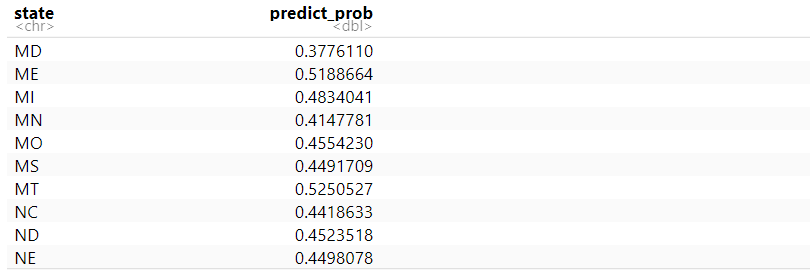
\includegraphics{/cloud/project/prob1.PNG}
\caption{Figure.12}
\end{figure}

\begin{figure}
\centering
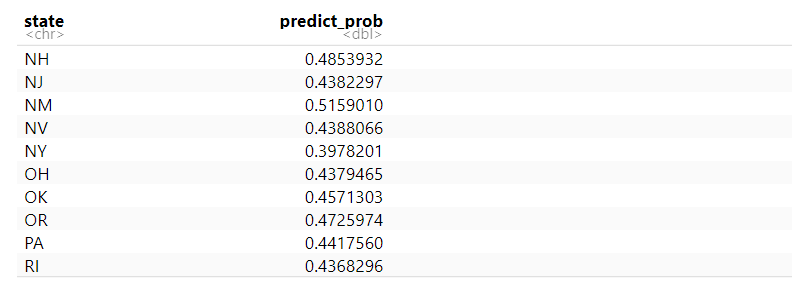
\includegraphics{/cloud/project/prob2.PNG}
\caption{Fig.13}
\end{figure}

\begin{figure}
\centering
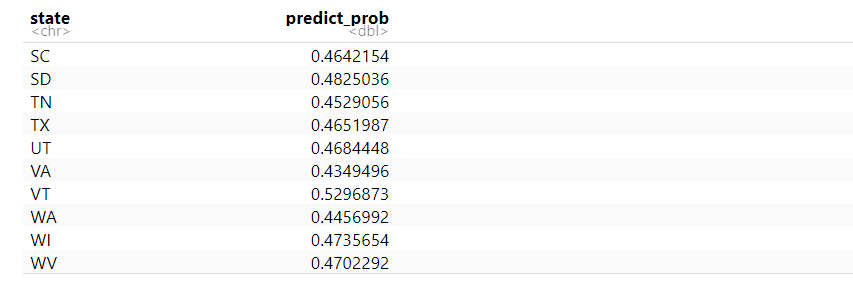
\includegraphics{/cloud/project/prob3.PNG}
\caption{Fig.14}
\end{figure}

\hypertarget{discussion}{%
\section{Discussion}\label{discussion}}

Our multilevel regression model with post-stratification implied three
results: 1) Maine (51.8\%), Montana (52.5\%), New Mexico (51.5\%) and
Vermont (52.9\%) have the highest probability of voting Trump in
electoral college; 2) the non-white voters tend to not vote for Trump,
since the estimated slope for people who are black or other races were
negative; 3) people in age group 24\textasciitilde29 do not have a
significant relationship with voting trump, this means that they are
less likely to vote for Trump.

Among these findings, the probability of voting Trump in each state was
especially worth mentioning. The voting system in the U.S. indicates
that 538 votes are allocated in the electoral college, which are based
on states' representation in Congress, this means that winning a
majority of votes is not enough, it is also important to win the votes
from swing states. In the past five elections, there were two elections,
including the 2016 Trump vs.~Clinton election, encountered the situation
in which the candidate won the majority of vote did not win the election
because they did not maintain their winning seat in electoral college
vote (Economist, 2020). Is 2020 election the same case as 2016 election?
This is the question we need to ask and investigate. From the model
results, we took extra attention on the swing states statistics, and
found that the probability of voting Trump in swing states such as
Arizona, Minnesota, Florida, were 47.9\%, 41\% and 46.7\% respectively.
It seems that Trump lost the majority of vote, but might also lose the
electoral college vote as well. However, this still remains uncertain
since the voting process is not yet finished, there might be changes in
the statistics at the end of the day. Our second finding was that
non-white voters tend not to vote for Trump, in other words, a majority
of Trump voters were whites. The past research showed that electoral
college favours white voters, such that the white share of voting power
is about 79\% (Economist, 2020). This is an extremely high number, and
Trump's supporters happened to be mainly whites. This implies that the
election outcome this year might be the same with the 2016 election,
since Trump might win a majority in electoral college again.

Although our model provides a prediction on the possibility of Trump
winning the election, we are only assuming this model is an accurate
description of the real world. This means that in real world, there are
too many factors that have the ability to alter the final election
outcome. In 2016 election, Nate Silver used predictive model to
calculate the winning chance of Clinton was 71\%, however, this does not
mean that his model was inaccurate or ``wrong'' (Breur, 2016). It only
means that in the statistical world, everything is based on the
information that was given, a high possibility on future event does not
imply certainty (Breur, 2016). A research finding helps illustrate this:
the voting system of the U.S. suggests that the location of the voters
can dramatically influence his/her voting power (Economist, 2020). As
the research states, ``a Granite Stater who moves to neighbouring
Vermont becomes 1,000 times less likely to affect the result of the
election, simply by moving a few miles.'' (Economist, 2020). This means
that the survey data and census data used in this report might be
actually outdated because we do not know how many people move to another
state, and how this might change the final voting power of the state.
There are also many other factors that could influence the future
outcomes, such as the role of social media, changes in voting behaviour.
Therefore, the findings resulted from the model in this report only
provide an insight to the election outcome. \# Weakness and Next Step
There are several weaknesses in our research. During the sample
selecting process, we were forced to narrow down our sample range by
about 100,000 people because the computer we used could not support
Rstudio to run such large amount of data. Our sample size might be too
small that there is a chance it affected the model accuracy and
reliability.

For future research, it is best to increase the sample size and select
more variables for the model. Also, researchers could try several models
and then pick the best one from them. In this report, we did not include
model selection process due to a lack of time, this should be fixed in
the future.

\hypertarget{appendix}{%
\section{Appendix}\label{appendix}}

Code for this analysis is available at:
\url{https://github.com/JessieZ32/2020_US_election}

\hypertarget{reference}{%
\section*{Reference}\label{reference}}
\addcontentsline{toc}{section}{Reference}

\hypertarget{refs}{}
\leavevmode\hypertarget{ref-citeCar}{}%
Fox, John, and Sanford Weisberg. 2019. \emph{An R Companion to Applied
Regression}. Third. Thousand Oaks CA: Sage.
\url{https://socialsciences.mcmaster.ca/jfox/Books/Companion/}.

\leavevmode\hypertarget{ref-citelabelled}{}%
Larmarange, Joseph. 2020. \emph{Labelled: Manipulating Labelled Data}.
\url{http://larmarange.github.io/labelled/}.

\leavevmode\hypertarget{ref-citeR}{}%
R Core Team. 2020. \emph{R: A Language and Environment for Statistical
Computing}. Vienna, Austria: R Foundation for Statistical Computing.
\url{https://www.R-project.org/}.

\leavevmode\hypertarget{ref-citeCodeMRP}{}%
Rohan Alexander. 2020. ``Getting Started with Mrp.''

\leavevmode\hypertarget{ref-citeACS}{}%
Steven Ruggles, Ronald Goeken, Sarah Flood, and Matthew Sobek. n.d.
\emph{IPUMS Usa: Version 10.0 {[}Dataset{]}}. Minneapolis, MN: IPUMS,
2020. \url{https://doi.org/10.18128/D010.V10.0}.

\leavevmode\hypertarget{ref-citeDFsurvey}{}%
Tausanovitch, Chris, and Lynn Vavreck. 2020. Democracy Fund + UCLA
Nationscape, October 10-17, 2019 (version 20200814). Retrieved from
{[}https://www.voterstudygroup.org/publication/nationscape-data-set{]}.

\leavevmode\hypertarget{ref-citeggplot2}{}%
Wickham, Hadley. 2016. \emph{Ggplot2: Elegant Graphics for Data
Analysis}. Springer-Verlag New York.
\url{https://ggplot2.tidyverse.org}.

\leavevmode\hypertarget{ref-citetidyverse}{}%
Wickham, Hadley, Mara Averick, Jennifer Bryan, Winston Chang, Lucy
D'Agostino McGowan, Romain François, Garrett Grolemund, et al. 2019.
``Welcome to the tidyverse.'' \emph{Journal of Open Source Software} 4
(43): 1686. \url{https://doi.org/10.21105/joss.01686}.

\leavevmode\hypertarget{ref-citehaven}{}%
Wickham, Hadley, and Evan Miller. 2020. \emph{Haven: Import and Export
'Spss', 'Stata' and 'Sas' Files}.

\end{document}
